\section{Planning with Clearance Value Annotations}
\label{aha:annotations}
In order to meet our stated goal of building a planner able to solve problems involving many degrees of heterogeneity we must first consider how to create an information-rich representation of the environment. We propose map annotation as the underpinning insight into solving this class of problem. \\ \newline
One way to overcome these issues  we need some way to identify the maximal obstacle distance for each map tile in our environment. We will measure this topographical feature by using a \emph{clearance value} metric. \\ \newline
A clearance value is associated with a tile on our grid map and represents the dimensions of a theoretical square bounding box that begins at the tile being evaluated and extends diagonally down and to the right \footnote{We assume down and right correspond to south and east on our grid map} until it intersects a hard obstacle or detects some change in the topograpy of the environment (we will expand on this idea a little later). This is an important measurement because it guarantees that the area subsumed by the bounding box is homogenous (topographically speaking). \\ \newline
Before delving any further, it is important to highlight two key assertions we make when computing tile clearance:
\begin{enumerate}
\item{Map tiles marked as non-traversable have a clearance value of 0.}
\item{Each traversable tile has a minimum clearance of 1; we will refer to this value as the \emph{base clearance}}.
\end{enumerate}
A simple method to recursively derive clearance is given by the following formula:
\begin{equation}
CV(t) = min(CV(t_{East}), CV(t_{South}), CV(t_{Southeast}))+BaseClearance
\end{equation}
Where:
\begin{itemize}
\item{$t$ is a traversable tile in our grid map.}
\item{$CV$ is the clearance value function which returns zero for all non-traversable tile parameters.}
\item{ $t_{East}$, $t_{South}$ and $t_{Southeast}$ are also tiles in our grid map (not necessarily traversable)\; their  subscripts indicate they are octile neighbours of $t$ in the stated directions.}
\end{itemize}
Undefined tiles -- those outside the grid map -- are, like hard obstacles, considered to have a clearance value of 0. This simple rule helps us deal with calculating clearance for traversable tiles along the border of a map. We illustrate these ideas in Figure \ref{effp-fig:calculatingclearance}.

\begin{figure}[htbp]
        \caption{\emph{Determining maximal clearance} (a): Each tile has a minimum base clearance of 1. (b) Clearance values for two adjacent traversable tiles on the map perimiter (c) Clearance values for a 3x3 traversable area. (d): The effect of a non-traversable neighbour on clearance. }
        \begin{center}
                        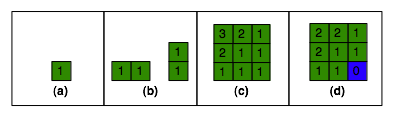
\includegraphics[scale=0.7]{diagrams/calculatingclearance.png}
        \end{center}
        \label{effp-fig:calculatingclearance}
\end{figure}

Once we have derived a clearance value, we use an additional few bytes of memory to annotate the corresponding node in our graph. This will allow us to better evaluate nodes when searching for a path.\\ \newline
Until now we have limited our discussion to computing clearance for a single terrain. This would work well if our agents were limited to traversing only one type of terrain (for example, a nautical agent is almost always waterbound) but we would like a more general solution to facilitate navigation for multi-capable units that can traverse many terrain types. We therefore need to compute and store several different clearance values -- one for each combination of terrains possible in our grid map. This process is identical to that described until now with only one major difference: we need to specify a target terrain parameter which we use to calculate the right clearance value. During processing, any tile we encounter that has a terrain type which is not a subset of the target terrain is regarded as soft obstacle and we assign it a clearance value of 0 for the target terrain. We continue in this manner until all map tiles have been processed. Figure \ref{effp-fig:annotations} shows the results of different clearance value annotations we embedded into a tiny map during development.
\begin{figure}[htbp]
        \caption{\emph{Single terrain and multi-terrain clearance value annotations.} Top: Clearance values for the single-terrain case. Bottom: Multi-terrain (Plains + Forests) annotations. In both cases, clearance values for hard-obstacles (here, water tiles) is omitted.}
        \begin{center}
                        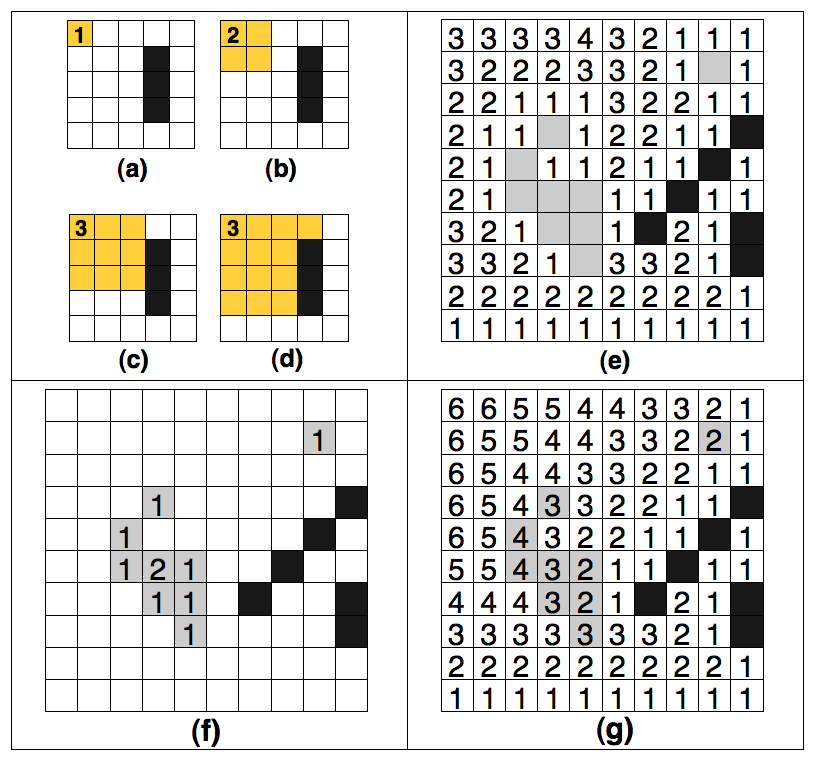
\includegraphics[scale=0.8]{diagrams/annotations.png}
        \end{center}
        \label{effp-fig:annotations}
\end{figure}
The exact number of clearance value annotations required for each map node is given by:
\begin{equation}
2^n - n
\label{effp-eq:cv}
\end{equation}

Where $n$ is the number of terrains on the map. \\ \newline
Since each node in our annotated graph represents a tile in the environment and each tile can only ever have a single terrain type it logically follows that we don't need to store annotations  for every distinct single-terrain type in every graph node. We also do not need to store annotations for the no-terrain case; thus deriving the result presented in equation \ref{effp-eq:cv}. Depending on the specific implementation and type of map overlay used, an additional annotation may also be required to store the terrain type of every tile. In our case, this was provided by the pathfinding library we used and we did not count it as extra overhead.\\ \newline
Using our definitions from above we are can easily produce a linear-time algorithm to generate our annotated graph; we present such an implementation in algorithm \ref{alg_annotatemap} and \ref{alg_ccv}. Since our implementation is recursive, we begin by calculating clearance with the first tile located at the map origin, (0,0).
\input content/alg1_calculateclearance
